\documentclass[]{article}
\usepackage[spanish]{babel} 
\usepackage{amsmath} 
\usepackage[colorlinks=true]{hyperref}
\usepackage{enumitem} 
\usepackage{graphicx}   
\usepackage[a4paper,top=2.5cm,bottom=2.5cm,left=2cm,right=2.5cm]{geometry} 
\usepackage[]{subfigure}
\usepackage[]{multicol}
\setlength{\columnsep}{1cm}
\usepackage[]{hyperref}
%\usepackage[maxbibnames=99, sorting=none]{biblatex}
\usepackage{amssymb}
\usepackage[]{txfonts}

%\usepackage[authoryear]{natbib}
\newenvironment{Figura}
{\par\medskip\noindent\minipage{\linewidth}}
{\endminipage\par\medskip}



%==================================================================================
\begin{document}
\begin{titlepage}
      \begin{center}     
              
            
\includegraphics[width=0.2\textwidth]{img/escudo_udec.png}                       %Para poner logo udec   %{nombre carpeta\nombreimagen}
            
            
            
            \vspace{1cm}
            \textsc{{\LARGE Universidad de Concepción}}
            
            \vspace{1cm}
            {\scshape\Large Facultad de ciencias fisícas y matemáticas \par}
            \vspace{2cm}
            {\scshape\Huge Laboratorio 3 \par}
            \vspace{2cm}
            {\itshape\Large Proyecto laboratorio termodinámica \par}
            \vfill
            {\Large Autores: \par}
            {\Large Martina Contreras, Noemí De La Peña, Benjamín Opazo. \par}
            \vfill
            \vfill
            {\Large Profesor: \par}
            {\Large Juan Pablo Staforelli \par}
            \vfill
            \vfill
            {\Large Carrera: \par}
            {\Large Ciencias fisícas \par}
            \vfill
            \vfill
            {\Large Ayudante: \par}
            {\Large Fernanda Paz Vera \par}
            \vfill
            {\Large Noviembre 2022 \par}
      \end{center}
\end{titlepage}            
 

\tableofcontents
\newpage



%==================================================================================



\begin{abstract}
  En este laboratorio se llevaron a cabo 4 experimentos relacionados con los circuitos eléctricos, donde se hizo variar el voltaje de entrada para estudiar la variación de la intensidad de corriente en cada circuito.
Los circuitos utilizados fueron: Conductor metálico, Filamento de ampolleta de linterna, Diodo semiconductor común y Diodo emisor de luz (DEL o LED).
Donde se concluye que cada material posee distintas propiedades, las cuales son: Potencia disipada, Conductividad o Resistividad y libre flujo de corriente.
\end{abstract}



%========Introducción=============
\section{Introdución}
Los primeros pasos para la creación de circuitos eléctricos fueron dados por el químico Alessandro Volta y la creación de la primera pila moderna. Ese fue el punto de partida básico para la   utilización práctica de la energía eléctrica, pasando a través de circuitos para cumplir diferentes finalidades.
Más tarde, hacia 1826, sería Georg Simon Ohm quien sentara las bases del estudio de la circulación de las cargas eléctricas en el interior de materias conductoras y formula la ley que relaciona las tres magnitudes más importantes: voltaje, intensidad y resistencia.
En este informe, primero definiremos conceptos claves para entender que es un circuito, tales como: Voltaje, Intensidad y resistencia. Luego presentaremos los materiales y procedimientos utilizados y un análisis para cada circuito utilizado, para concluir con lo que hemos aprendido en este laboratorio.


%==============Marco teorico============
\section{Marco teórico}

  \textbf{La Corriente eléctrica,} expresada como un flujo de partículas, se escribe:
  \begin{align*}
    I = \int_{A} J\cdot  dS
  \end{align*}
  donde: \\
    $J = \sum_{i} n_i \, q_i \langle v_i\rangle$ es el \textbf{vector densidad de corriente}, la cual expresa
    la contribución de los eventuales varios portadores de carga participantes en el proceso de condución eléctrica,
    dependiendo de la clase de material de que se trate. En la conducción metálica, los portadores son electrones solamente, entonces,
    \begin{align*}
      J = n_i \, e\mu E
    \end{align*} 
  donde $n, e, \mu$ expresan la concentración (número/volumen), la carga y la movilidad de los electrones, respectivamente,
  cuando hay aplicado un campo eléctrico \textbf{E}. Definimos $\sigma = n_i \, e\mu$ como la conductividad del material conductor en estudio y 
  $\rho = \frac{1}{\sigma}$ su resistividad. \\

  Para un trozo de conductor cilíndrico, de área transversal $A$ y longitud $l$, su resistencia eléctrica $R$ queda expresada
  por: 
  \begin{align*}
    P = I^2 \, R = V \, I = \frac{V^2}{R}
  \end{align*} 
  Esta relación expresa la rapidez con que se fectuá la transformación o potencia desarrollada. \\
  
  La teoría de conducción eléctrica en semiconductores, considera dos clases de portadores de carga, electrones
  con carga $(-e)$ y huecos con carga $(+e)$. Ambos tipos tienen igual concentración cuando el semiconductor está en estado
  puro (intrínseco). Por métodos físico-químicos se pueden incorporar átomos de otros elementos ('impurezas') que permiten
  hacer que una u otra de las concentraciones de portadores predomine. Si predominan los portadores de carga $(-)$ se habrá 
  obtenido un semiconductor tipo $n$ y de tipo $p$, llamada unión $p - n$. Las propiedades de una unión $p-n$ se verán reflejadas en la curva característica
  I vs V de los diodos.

  \begin{itemize}
    \item \textbf{Voltaje\cite{voltaje}: } El voltaje es la diferencia de potencial eléctrico entre dos puntos de un circuito eléctrico o electrónico, expresado en voltios. 
    Mide la energía potencial de un campo eléctrico para provocar una corriente eléctrica en un conductor eléctrico.
  \end{itemize}




%=========Materiales===============
\section{Materiales}

  \begin{itemize}
    \item Conductor metálico (fino alambre de metal).
    \item Filamento de ampolleta de linterna.
    \item Diodo semiconductor común.
    \item Diodo emisor de luz (DEL o LED).
    \item Una fuente de poder electrónica (FPE).
    \item Dos multímetros digitales.
    \item Siete cables de conexión.
  \end{itemize}

%================Procedimiento=================================
\section{Procedimiento}
\begin{enumerate}

  \item  Ubicamos los selectores de M1 y M2 en 40(DCV) y 2 (DCA), respectivamente. Ahora, conectamos M1, y M2.
Instalamos como elemento X el \textbf{conductor metálico}, conectándolo entre P y Q. La corriente máxima que 
se hará circular será de 0.50 A. 
Luego, hacemos 10 medidas en el rango (0.00 - 0.50)(A) para cada polaridad. Una vez que tomamos los datos, desconectamos
el terminal \textbf{(+)} de la \textbf{FPE} y accionamos el control para volver a $0 V$ en la fuente. \\


\item Cambiamos el elemento X, instalando ahora la \textbf{ampolleta de la linterna.} Volvemos a conectar el terminal $(+)$ de la FPE. 
Para no dañar su filamento, conviene seleccionar un rango apropiado de corrientes. Se nos recomienda utilizar los
siguientes valores en la escala de $400 mA$ (DCA) de M2: 20; 40; 60; 80; 100; 120; 160; 180; 200. Mantenemos M1 en 
su escala. Aquí también efectuamos la inversición de polaridad, para cada valor de corriente. Denuevo, al finalizar la serie,
desconectamos el terminal (+) y retornamos a $0 (V)$ la FPE.

\item A continuación, cambiamos el elemento X, instalando el diodo \textbf{semiconductor común.} Reinstalamos la conexión
del terminal $(+)$ de la FPE. Ahora, trabajaremos separadamente las polaridades directa e inversa. Con polarizacion directa,
ajustamos los siguientes valores de corriente en la escala de 2 A (DCA): 0.050; 0.080; 0.100; 0.120; 0.130;
0.140; 0.160; 0.200; 0.250; 0.300; 0.350; 0.400. Iniciamos el control de voltaje de manera cuidadosa, desde 0.00 V hasta
0.60 V. De ahí en adelante extremamos las precauciones ajustando sólo con el control fino. Tratamos de definir el llamado
voltaje de arranque del diodo, donde se hace bruscamente conductor. Luego, cambiamos a polaridad inversa
y exploramos hasta donde sea posible; valores altos de voltajes son permitidos, en tanto la corriente se mantenga baja. Efectuamos 10 
medidas para cada polaridad. Finalmente, desconectamos el terminal (+) y retornamos a 0 (V) la salida de la fuente.


\item  Instalamos el diodo emisor de luz. Restauramos la conexión (+) de la fuente y comenzamos a incrementar el voltaje
hasta 1.50 V en una primera etapa. Luego, prestamos más atención a los valores de corriente ajustando con el control 
fino de voltaje 10 pares de valores $I^{+}$, $V^{+}$ con corrientes comprendidas en el rango: 0.20 (mA), hasta 5.00 (mA)
en la escala de 40 (mA) (DCA). Luego, tratamos de ubicar el punto de encendido del LED, visualmente y anotamos dicho valor; efectuamos
10 medidas $I^{+}$, $V^{+}$ para la polaridad. Además, realizamos mediciones con polaridad inversa con el LED. \\

\includegraphics[width=8cm, height=5cm]{img/circuito.jpg}
\end{enumerate}

% \begin{figure}
%   \centering
%   \includegraphics[width=12cm, height=8cm]{img/circuito.jpg}
% \end{figure}

\begin{table}
  \centering
  \begin{tabular}{|c|c|c|c|c|} \hline
    dato    &   $V^{+}$ [v]  &    $I^{+}$[A]  &   $V^{-}$ [v]  &    $I^{-}$ [A]  \\ \hline
    1       & 0.02 &0.01   &-0.56 &-0.05 \\ \hline
    2      &0.28  &0.02     &-0.74 &-0.07 \\ \hline
    3      &0.45  &0.03     &-1.35 &-0.12 \\ \hline
    4       &0.73  &0.07    &-1.76 &-0.17 \\ \hline
    5       &0.99  &0.09    &-2.23 &-0.22 \\ \hline
    6       &1.42  &0.14    &-2.66 &-0.27 \\ \hline
    7       &2.63  &0.26    &-3.42 &-0.35 \\ \hline
    8       &3.71  &0.37    &-3.97 &-0.41 \\ \hline
    9       &4.13  &0.42    &-4.29 &-0.44 \\ \hline
    10       &4.82  &0.49   &-4.92 &-0.5 \\ \hline

  \end{tabular}
  \caption{\label{tab: transitor} Conductor metálico}
\end{table}






\begin{table}
  \centering
  \begin{tabular}{|c|c|c|c|c|} \hline
    dato    &   $V^{+}$ [v]  &    $I^{+}$[A]  &   $V^{-}$ [v]  &    $I^{-}$ [A]  \\ \hline
    1& 0.10 &0.01 &-0.05& 0.00 \\ \hline
    2&0.31 &0.02  &-0.09& 0.01 \\ \hline
    3&0.71 &0.03 &-0.18& 0.02 \\ \hline
    4&0.81 &0.04 &-0.39& 0.03 \\ \hline
    5&1.09 &0.05 &-0.89& 0.04 \\ \hline
    6& 1.49 &0.06 &-1.15& 0.05 \\ \hline
    7& 1.72 &0.07 &-1.60& 0.06 \\ \hline
    8& 2.01 &0.08 &-2.03& 0.07 \\ \hline
    9& 2.90 &0.09  &-2.56& 0.08 \\ \hline
    10& 3.64 &0.10 &-3.26& 0.10 \\ \hline
    
    
  \end{tabular}
  \caption{\label{tab: ampolleta} Ampolleta de linterna. }
\end{table}



\begin{table}
  \centering
  \begin{tabular}{|c|c|c|c|c|} \hline
    dato    &   $V^{+}$ [v]  &    $I^{+}$[A]  &   $V^{-}$ [v]  &    $I^{-}$ [A]  \\ \hline
    1&0.67& 0.00&     -0.40& 0.00\\ \hline
    2&0.68& 0.00&     -1.98& 0.00\\ \hline
    3&0.70& 0.00&     -4.08& 0.00\\ \hline
    4&0.71& 0.00&     -6.53& 0.00\\ \hline
    5&0.72& 0.00&     -7.35& 0.00\\ \hline
    6&0.73& 0.01&     -8.41& 0.00\\ \hline
    7&0.74& 0.02&     -9.23& 0.00\\ \hline
    8&0.75& 0.03&     -10.08& 0.00\\ \hline
    9&0.76& 0.04&     -11.41& 0.00\\ \hline
    10&0.76& 0.04&     -12.62& 0.00 \\ \hline
    
    
  \end{tabular}
  \caption{\label{tab: diodo-comun} Diodo semiconductor común.}
\end{table}


\begin{table}
  \centering
  \begin{tabular}{|c|c|c|c|c|} \hline
    dato    &   $V^{+}$ [v]  &    $I^{+}$[A]  &   $V^{-}$ [v]  &    $I^{-}$ [A]  \\ \hline
    1&0.00& 0.00&     -0.93	&0.00\\ \hline
    2&1.43& 0.00&     -2.17	&0.00\\ \hline
    3&1.80& 0.00&     -3.42	&0.00\\ \hline
    4&2.40& 0.01&     -4.42	&0.00\\ \hline
    5&2.56& 0.01&     -5.62	&0.00\\ \hline
    6&2.65& 0.02&     -7.46	&0.00\\ \hline
    7&2.80& 0.02&     -8.84	&0.00\\ \hline
    8&2.95& 0.02&     -10.21	&0.00\\ \hline
    9&3.01& 0.03&     -11.00	&0.00\\ \hline
    10&3.35& 0.04&     -12.22	&0.00\\ \hline
    
    
  \end{tabular}
  \caption{\label{tab: emisor-luz} Diodo emisor de luz.}
\end{table}

\begin{figure}
  \centering
  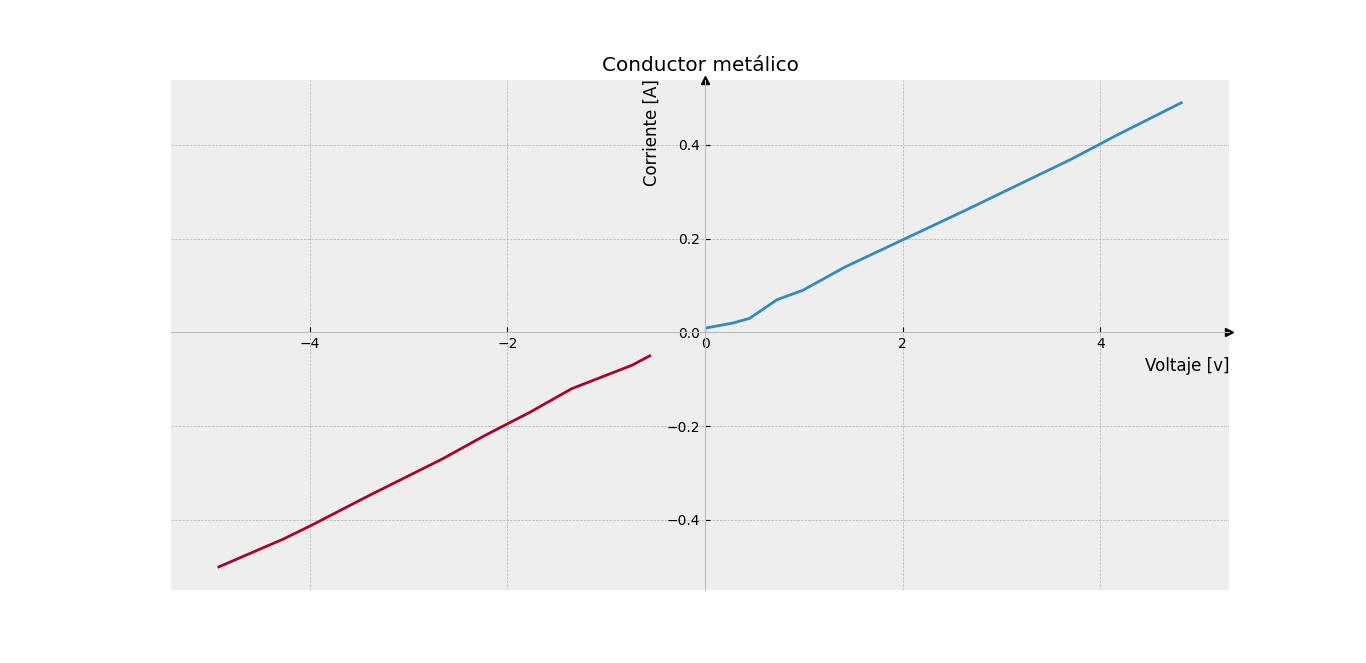
\includegraphics[width=12cm, height=8cm]{img/Figure_2.png}
  \caption{\label{fig: fig-conductor}Gráfico de conductor metálico.} 
\end{figure}

\begin{figure}
  \centering
  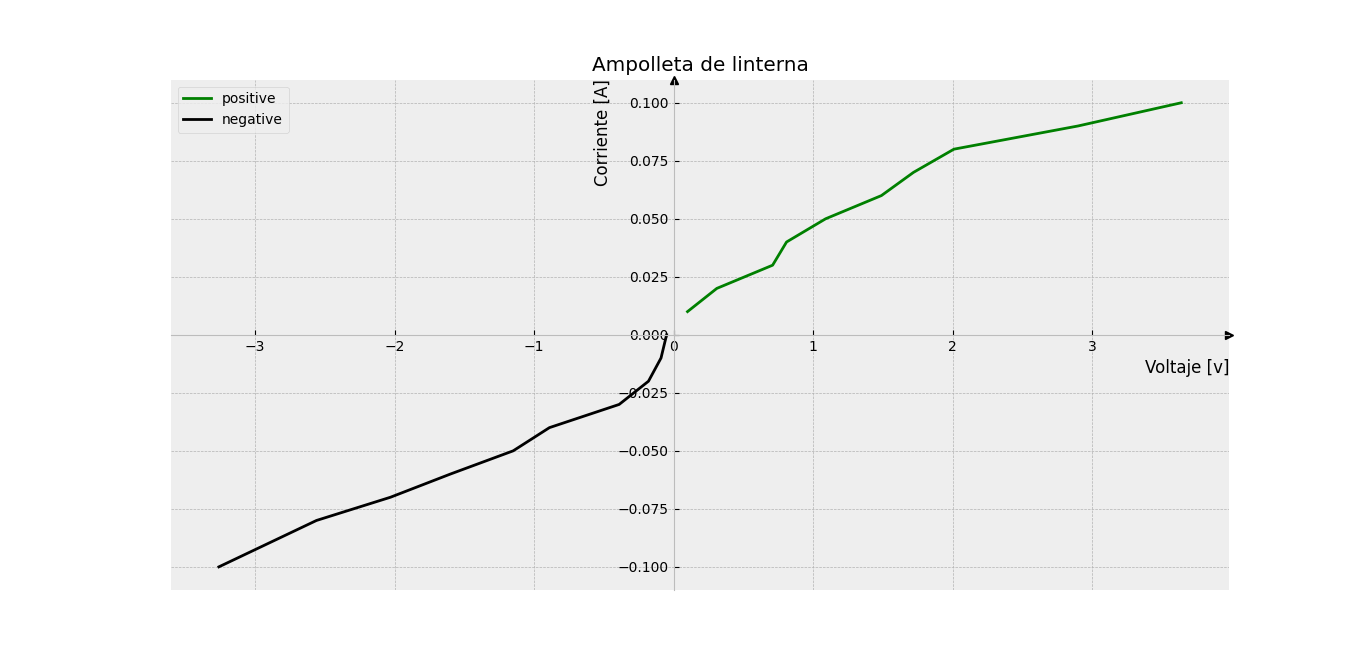
\includegraphics[width=12cm, height=8cm]{img/Figure_1.png}
  \caption{\label{fig: fig-ampolleta}Gráfico ampolleta de linterna.} 
\end{figure}

\begin{figure}
  \centering
  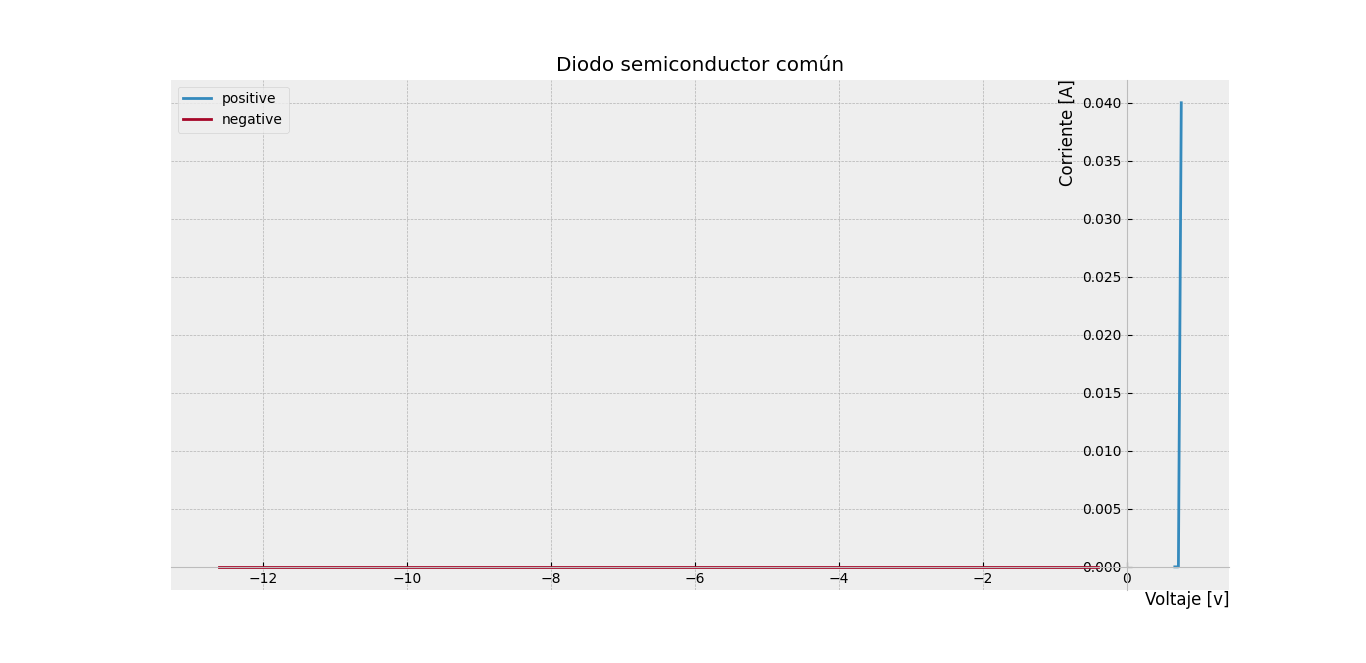
\includegraphics[width=12cm, height=8cm]{img/Figure_3.png}
  \caption{\label{fig: diodo-comun}Gráfico diodo semicondor común $(+)$.} 
\end{figure}

\begin{figure}
  \centering
  \includegraphics[width=12cm, height=8cm]{img/Figure_4.png}
  \caption{\label{fig: emisor-luz}Gráfico diodo emisor de luz $(+)$.} 
\end{figure}








%============Análisis==========================================================
\section{Análisis}
Vemos que para el primer gráfico \ref{fig: fig-conductor} de I v/s V, donde el circuito está conectado a un conductor metálico, tiene un comportamiento lineal, y para el lado de la corriente directa e inversa el gráfico de los datos es casi idéntico, por lo que I y V están relacionados de manera lineal por la ley de Ohm %aqui hacer alguna referencia a una ecuacion que corresponda a la ley de Ohm  
,además de que los conductores metálicos tienen una alta conductividad eléctrica y por ende poca resistividad, por lo que la potencia que disipan en forma de calor es mínima.\\

Para el circuito conectado a la ampolleta de linterna, notamos que su gráfico \ref{tab: ampolleta} I vs V tiene un comportamiento distinto al del conductor metálico se nota que hay una relación entre la corriente y el voltaje, pero ya no es lineal, por lo que la relación entre las dos no puede ser explicada por la ley de Ohm, por ende, la ampolleta de linterna tiene una conductividad eléctrica menor que el conductor metálico y por ende una mayor resistencia, de lo cual concluimos que hay una mayor disipación de calor, al transformar la corriente que circula en energía eléctrica, la cual es la que produce que en algún momento la ampolleta de linterna se prenda y aumente de a poco su brillo hasta llegar a un límite.\\

Para el circuito conectado al diodo semiconductor común vemos que, al igual que el gráfico de la ampolleta de linterna, el gráfico  \ref{fig: diodo-comun} de I v/s V tiene un comportamiento lineal hasta un cierto punto de voltaje y luego la corriente cambia rápidamente, donde vemos que, en el caso donde la corriente es directa, a medida que aumenta el voltaje la corriente casi no cambia de manera visible en 0.00, por un largo intervalo de voltaje, no obstante, cambiaba de manera más pequeña que eso, ya que el instrumento que usabamos no tenía la sensibilidad para poder detectar esos pequeños cambios, hasta que para un cierto valor de voltaje que en nuestro caso fue de 0.73 V empieza a cambiar la corriente de manera notoria por lo que entre 0.73 V y 0.76 V es el voltaje de arranque, y que además, a medida que aumenta más la corriente el voltaje se mantiene constante con una valor de 0.76, también vemos que cuando la corriente es inversa el diodo semiconductor común se convierte en un aislante ya que la corriente se matiene en 0.00 sin importar el valor del voltaje, y ya que se convierte en un aislante, su resistividad eléctrica es mayor y por ende su resistencia también.\\

Para el circuito conectado al diodo emisor de luz vemos que, al igual que el gráfico del diodo semiconductor común este \ref{fig: emisor-luz} tiene un comportamiento lineal al inicio, cuando la corriente es directa, porque al principio no pasa una cantidad de corriente notoria, y el instrumento no puede detectarla, pero luego la corriente que pasa aumenta y sigue aumentando, a diferencia del diodo semiconductor común, este no tiene un comportamiento donde el voltaje no aumenta o se mantiene casi constante, sino que este sigue aumentando, es decir se vuelve en un conductor, pero como este transforma energía eléctrica en luz, para que se pueda prender el diodo y llegue a un límite, disipa potencia en forma de calor, y hace que el voltaje tammbién cambie, como el conductor metálico. En el caso donde la corriente es inversa podemos ver que al igual que el diodo semiconductor común, el diodo emisor de luz se transforma en un aislante, ya que no permite el flujo de corriente, y por ende nunca se ilumina, por lo que su resistividad eléctrica es mayor, y por consecuencia su resistencia también. 



%============Conclusión========================================================
\section{Conclusión}
De los 4 experimentos realizados, se logra concluir que:
Primero, de que cuando no existe una relación lineal entre $V$ (voltaje) y $I$ (intensidad), el circuito posee una conductividad menor. Además, que a mayor conductividad tenga un circuito, menor será el potencial que disipa en forma de calor. 
También  logramos percibir que los circuitos compuestos por diodo poseen la característica de volverse aislantes, cuando son conectados a un voltaje de cargas negativas.
Por otro lado, los diodos en corriente directa al sobrepasar el voltaje de arranque se vuelven en un buen conductor, notar que esto se cumple
solamente para el \textbf{diodo semiconductor común.} Además, para el caso diodo emisor de luz y ampolleta de linterna, estos transforman la energía eléctrica en energía lumínica, y por consecuencia,
disipaban potencia en forma de calor.

\begin{thebibliography}{5}
  \bibitem{voltaje} Medidas de voltaje: Guía. (s. f.). NI. Recuperado 4 de noviembre de 2022, 
  de \url{https://www.ni.com/es-cl/support/documentation/supplemental/21/how-to-measure-voltage.html}
  \bibitem{Noe}Corriente eléctrica y materiales conductores. (2014, 5 septiembre). RedUSERS. 
  \url{https://www.redusers.com/noticias/corriente-electrica-y-materiales-conductores/}
  \bibitem{libro} \textbf{D. Halliday; R. Resnick; K. S. Kane.} \textit{Física Vol. 2.} (Cap.32), Compañía Editorial Continental, S.A. de C.V. 3º Edición, 1994
  \bibitem{benja} Circuito Eléctrico: Historia. (s. f.). Recuperado 4 de noviembre de 2022,
   de \url{https://www.profesorenlinea.cl/mediosocial/Circuito_ElectricoHistoria.htm}
\end{thebibliography}




\end{document}